\documentclass[12pt,utf8,notheorems,compress]{beamer}

\usepackage[utf8]{inputenc}
\usepackage{default}

\usepackage{lmodern,listings}

% \usepackage{type1cm}
% \usepackage{type1ec}
% \RequirePackage{fix-cm}  %(Die Warnungen wurden schon durch lmodern beseitigt.)

% \usetheme{Berlin}
\usetheme{Warsaw}
\useoutertheme{split}
\usecolortheme{seahorse}
\usepackage{kurier}
\useinnertheme{rectangles}
\setbeamertemplate{navigation symbols}{}
\setbeamertemplate{footline}{}
\setbeamertemplate{headline}{}




% \usepackage[ngerman]{babel}
\usepackage[T1]{fontenc} % Trennung bei Woertern mit Umlauten
\usepackage{amssymb,amsmath,amsthm}
\usepackage{url,tikz}
\usepackage{graphicx}
\usepackage{comment,microtype}
\usepackage{listings}
\usepackage{pst-all}

%\usepackage{tikz-cd} % for commutative diagrams, but didn't work here
\usepackage{amsmath,amscd} % for (very simple) commutative diagrams

%\hyphenation{mani-fold}
%\hyphenation{sub-mani-fold}

\setlength\parskip{\medskipamount}
\setlength\parindent{0pt}

\newcommand{\slogan}[1]{%
  \begin{center}%
    \setlength{\fboxrule}{2pt}%
    \setlength{\fboxsep}{-3pt}%
    {\usebeamercolor[fg]{item}\fbox{\usebeamercolor[fg]{normal
    text}\parbox{0.9\textwidth}{\begin{center}#1\end{center}}}}%
  \end{center}%
}

% top color=#2!10, bottom color=#2!90

\newcommand{\mybox}[2]{%
         \begin{center}%
            \begin{tikzpicture}%
                \node[rectangle, draw=#2, rounded corners=5pt, inner xsep=5pt, inner ysep=6pt, outer ysep=10pt]{
                \begin{minipage}{0.75\linewidth}#1\end{minipage}};%
            \end{tikzpicture}%
         \end{center}%
}

\everymath{\displaystyle}

\title{Hacking Workshop -- Mathecamp 2016 in Windischleuba}

\author{Sven Prüfer}

%\institute{Institut f\"ur Mathematik, Universit\"at Augsburg}

\date{\today}

%\titlegraphic{
% \includegraphics[width=8cm]{./Uni_Aug_Logo_MNF_CMYK.pdf}
%}

\setlength{\unitlength}{1cm}

\begin{document}

\setbeameroption{show notes}
\setbeamertemplate{note page}[plain]

\begin{frame}
 \titlepage
\end{frame}

\begin{frame}[shrink=25]
%\frametitle{Inhalt}
\vspace{1cm}
\tableofcontents
\end{frame}

\section{Hinweise}

\begin{frame}
  \frametitle{Hinweise}
  \begin{center}
    \Huge Hinweise
  \end{center}
\end{frame}

  \begin{frame}
    \frametitle{Rechtliches}
    Macht niemals irgendsoetwas auf Rechnern, auf denen ihr das nicht dürft oder von deren Betreibern ihr kein Einverständnis habt.
    \pause \vfill
    Und auf gar keinen Fall in der Schule!
  \end{frame}

  \begin{frame}
    \frametitle{Praktisches}
    Viele Menschen wollen euch Böses!
    \pause \vfill
    Traut keinen zwielichten Websites, installiert niemals (besonders unter Windows) merkwürdige Programme!
    \pause \vfill
    Informiert euch unbedingt über Skripte und Programme, bevor ihr sie ausführt!
    \pause \vfill
    Vertrauenswürdige Websites sind insbesondere \textsc{stackoverflow.com}, \textsc{superuser.com} oder \textsc{news.ycombinator.com}.
  \end{frame}

\section{Linux}

\subsection{System}

\begin{frame}
  \frametitle{Linux}
  \begin{center}
    \Huge Linux -- System
  \end{center}
\end{frame}

\begin{frame}
  \frametitle{Dateistruktur}
  ``Alles ist eine Datei'' -- Grundprinzip von Unix
  \pause \vfill
  Das Wurzelverzeichnis ist ``/'' anstelle einer Partition (``C'' unter Windows).
  \pause \vfill
  Wichige Verzeichnisse sind insbesondere:
  \begin{tabular}{lc}
    /dev & Geräte \pause  \\
    /media & Medien \pause \\
    /home & Private Dateien der Nutzer \pause \\
    /etc & Konfigurationsdateien, insb. /etc/ssl \pause \\
    /var & Variable Dateien, insb. /var/www \pause \\
    /bin & Binäre Dateien \pause \\
    /tmp & Temporäre Dateien
  \end{tabular}
  
\end{frame}

\begin{frame}
  \frametitle{Benutzerrechte}
  Dateisystem speichert Lese-/Schreib-/Nutzungsrechte für jede einzelne Datei und jeden Ordner
  \pause \vfill
  Bedeutung von Rechten bei Verzeichnissen anders.
  \pause \vfill
  Bei guter Nutzung von Rechten kann Eindringling im besten Fall nichts machen.
  \pause \vfill
  Wichtigster Nutzer: \emph{root}
  \pause \vfill
  Beispiel in Konsole.
\end{frame}

\subsection{Kommandozeile}

% cd, ls, cat, man, |, pyhton+perl+etc

\begin{frame}
  \frametitle{Kommandozeile}
  \begin{center}
    \Huge Die Kommandozeile
  \end{center}
\end{frame}

\begin{frame}
  \frametitle{Terminal, Bash und Shell}
  Eine \emph{Shell} verarbeitet Kommandozeilenbefehle und gibt eine Antwort.
  \pause \vfill
  Die \emph{Bash} ist die bekannteste Shell. Es gibt noch viele andere.
  \pause \vfill
  Ein \emph{Terminal} ist eine Art Verpackung für eine Shell, also z.B.\ das Fenster in dem die Shell läuft.
\end{frame}

\begin{frame}
  \frametitle{Wichtigste Befehle}
  \begin{tabular}{ll}
    cd & Wechsle Verzeichnis \\
    ls & Zeige Verzeichnisinhalt \\
    cat & Zeige/Gib wieder Inhalt von Textdateien an \\
    man & Zeige Hilfe zu Befehl an \\
    python/perl/gcc & Kompiliere mit entsprechender Sprache \\
    sh & Führe Shellskript aus \\
    DATEI & Führe binäre DATEI aus \\
    make & Führe make Skript aus
  \end{tabular}
\end{frame}

\begin{frame}
  \frametitle{Pipes}
  Befehle in der Bash können hintereinander ausgeführt werden mittels einer Pipe ``|''. Diese gibt die Ausgabe als Eingabe an den nächsten Befehl weiter.
  \pause \vfill
  cat testdatei | uniq -u | sort
  \pause \vfill
  Gibt den Inhalt der Datei ``testdatei'' weiter an ``uniq'' mit Option ``-u'', doppelte Zeilen werden weggeschmissen und danach sortiert. 
\end{frame}

% \begin{figure}[H]
% \centering
% \includegraphics[width=0.5\linewidth]{parental_advisory.png}
% \end{figure}

% \begin{picture}(0,0)
%   \put(0,0){%
%     \includegraphics[scale=0.2]{fg1.jpg}
%    }
%    \put(6,0.5){%
%     \includegraphics[scale=0.2]{fg2.jpg}
%    }
%    \put(0,-4){%
%     \includegraphics[scale=0.2]{fg3.jpg}
%    }
%    \put(4.5,-4){%
%     \includegraphics[scale=0.2]{got_fight.jpg}
%    }
%    \put(8.5,-4){%
%     \includegraphics[scale=0.2]{book.jpg}
%    }
% \end{picture}

\section{Grundlagen Netzwerkkommunikation}

\begin{frame}
  \frametitle{Grundlagen Netzwerkkommunikation}
  \begin{center}
    \Huge Grundlagen Netzwerkkommunikation
  \end{center}
\end{frame}

\begin{frame}
  \frametitle{Schichtenmodell}
  \begin{figure}[H]
  \centering
  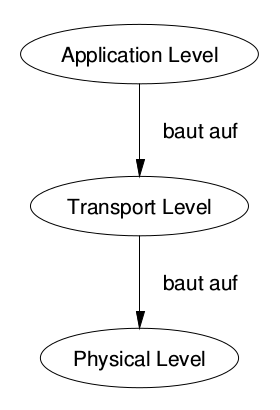
\includegraphics[width=0.5\linewidth]{osi.png}
  \end{figure}
\end{frame}

\begin{frame}
  \frametitle{RFC}
  RFC = Request for Comments
  \pause \vfill
  Internetstandards werden damit (in einfacher Textdatei) vorgeschlagen und zur Diskussion gestellt.
  \pause \vfill
  De facto werden Internetstandards damit definiert.
  \pause \vfill
  \begin{figure}[H]
  \centering
  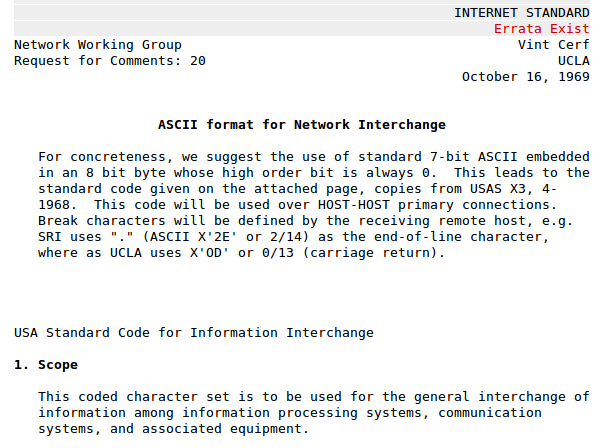
\includegraphics[width=0.5\linewidth]{rfc.png}
  \end{figure}
\end{frame}

\subsection{IPs und DNS}

\begin{frame}
  \frametitle{IPs und DNS}
  \begin{center}
    \Huge IPs und DNS
  \end{center}
\end{frame}

\begin{frame}
  \frametitle{IP-Protokoll}
  Grundlegendes Protokoll um Pakete vom Quell-Host zum Ziel-Host zu senden.
  \pause \vfill
  Pakete bestehen aus ``Header'' und ``Payload''.
  \pause \vfill
  Es existieren zwei wichtige Versionen: IPv4 und IPv6.
  \pause \vfill
  Beispiel:

  45 10 00 2C 24 B2 00 00 40 06 FD DF AC 10 00 09 AC 10 00 01 04 47 00 17 60 C6 DF 90 00 00 00 00 60 02 02 00 F9 46 00 00 02 04 05 B4

  Analyse etwas später!
\end{frame}

\begin{frame}
  \frametitle{Beispiel IPv4 Paket 1}
  Beispiel (jedes ``Paar'' sind zwei Hexadezimalzahlen, also jeweils vier Bit, also insgesamt 1 Byte) von Michael Egan:

  45 10 00 2C 24 B2 00 00 40 06 FD DF AC 10 00 09 AC 10 00 01 04 47 00 17 60 C6 DF 90 00 00 00 00 60 02 02 00 F9 46 00 00 02 04 05 B4
  \pause \vfill
  4 -- IPv4
  \pause \vfill
  5 -- Länge des IP Headers in 32-Bit-Wörtern $\Rightarrow$ 20 Bytes
  \pause \vfill
  10 -- Type of Service (?)
  \pause \vfill
  00 2C -- Länge des Pakets $\Rightarrow$ 44 Bytes
  \pause \vfill
  24 B2 -- Durchnummerierung der Pakete
  \pause \vfill
  00 00 (Verschiedene IP Flags)
  \pause \vfill
  40 -- ``Time to live''
  \pause \vfill
  06 -- Protokoll $\Rightarrow$ TCP
 \end{frame}

\begin{frame}
  \frametitle{Beispiel IPv4 Paket 2}
  45 10 00 2C 24 B2 00 00 40 06 FD DF AC 10 00 09 AC 10 00 01 04 47 00 17 60 C6 DF 90 00 00 00 00 60 02 02 00 F9 46 00 00 02 04 05 B4
  \vfill
  FD DF -- Checksum des IP-Headers
  \pause \vfill
  AC 10 00 09 -- Quell-IP-Adresse $\Rightarrow$ 172.16.0.9
  \pause \vfill
  AC 10 00 01 -- Ziel-IP-Adresse $\Rightarrow$ 172.16.0.1
  \pause \vfill
  Beginn TCP-Header: 04 47 -- Quellport $\Rightarrow$ 1095
  \pause \vfill
  00 17 -- Zielport $\Rightarrow$ 23 (Telnet)
  \pause \vfill
  60 C6 DF 90 -- Sequenznummer SEQ\#
  \pause \vfill
  00 00 00 00 -- Bestätigungsnummer ACK\# (normalerweise SEQ\# des vorherigen Pakets, hier aber erstes Paket)
  \pause \vfill
  6 -- Länge des TCP Headers in 32-Bit-Wörtern $\Rightarrow$ 24 Bytes
\end{frame}

\begin{frame}
  \frametitle{Beispiel IPv4 Paket 3}
  45 10 00 2C 24 B2 00 00 40 06 FD DF AC 10 00 09 AC 10 00 01 04 47 00 17 60 C6 DF 90 00 00 00 00 60 02 02 00 F9 46 00 00 02 04 05 B4
  \vfill
  0 02 -- TCP Flags (?)
  \pause \vfill
  02 00 -- Fenstergröße für sogenanntes ``Sliding Window Protocoll'' zum Verhindern vom Senden zuvieler Pakete
  \pause \vfill
  F9 46 -- Checksum TCP-Header
\end{frame}

\begin{frame}
  \frametitle{IP-Adressen}
  IPv4 nutzt 4 Bytes um Rechner zu adressieren, z.B. 5.189.172.46.
  \pause \vfill
  Notation: 192.0.2.0/24 bezeichnet alle Adressen 192.0.2.0 bis 192.0.2.255
  \pause \vfill
  Spezielle Adressen: \pause
  10.0.0.0/8, \pause 172.16.0/12, \pause 192.168.0/16 \pause
  \vfill
  IPv4-Adressen sind alle vergeben :-(
  \pause \vfill
  Aber es gibt IPv6! :-)
  \pause \vfill
  IPv6 nutzt 16 Bytes, typischerweise in Hexadezimal und ohne Nullen, z.B.
  2001:0DB8:AC10:FE01::::  
\end{frame}

\begin{frame}
  \frametitle{Routing}
  Rechner am Internet schicken nicht jedes Paket direkt an ihr Ziel
  \pause \vfill
  Stattdessen hat jeder Rechner eine \emph{Routing-Tabelle} und schickt Pakete nach einem Routingprotokoll.
  \pause \vfill
  \begin{figure}[H]
  \centering
  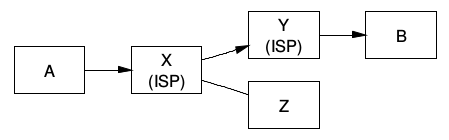
\includegraphics[width=0.75\linewidth]{routing-graph.png}
  \end{figure}
  \pause \vfill
  Vor 1993: IPs hierarchisch nach Größe der Netzwerke aufgeteilt (``classfull'') $\Rightarrow$ Riesige Routingtables und nicht genügend IPs für LANs
  \pause \vfill
  Nach 1993: CIDR $\Rightarrow$ Netzwerk- und Hostanteil der IP.
\end{frame}

\begin{frame}
  \frametitle{TCP 1}
  TCP = Transmission Control Protocol
  \pause \vfill
  Erweiterung von IP um \pause
  \begin{itemize}
    \item Fehlerkorrektur (Reihenfolge und Wiederholung) durch Nummerierung der Pakete \pause
    \item Ports \pause
    \item ``Verbindungsauf- und abbau''
  \end{itemize}
  \vfill \pause
  TCP hat eigenen Header, der innerhalb der IP-Payload liegt.
  \vfill \pause
  TCP regelt ``alles'' für die Anwendungen: Mittels TCP/IP werden Pakete verschickt bis alles vollständig und korrekt ist, erst dann erhält die Anwendung die Daten.
\end{frame}

\begin{frame}
  \frametitle{TCP 2}
  \begin{figure}[H]
  \centering
  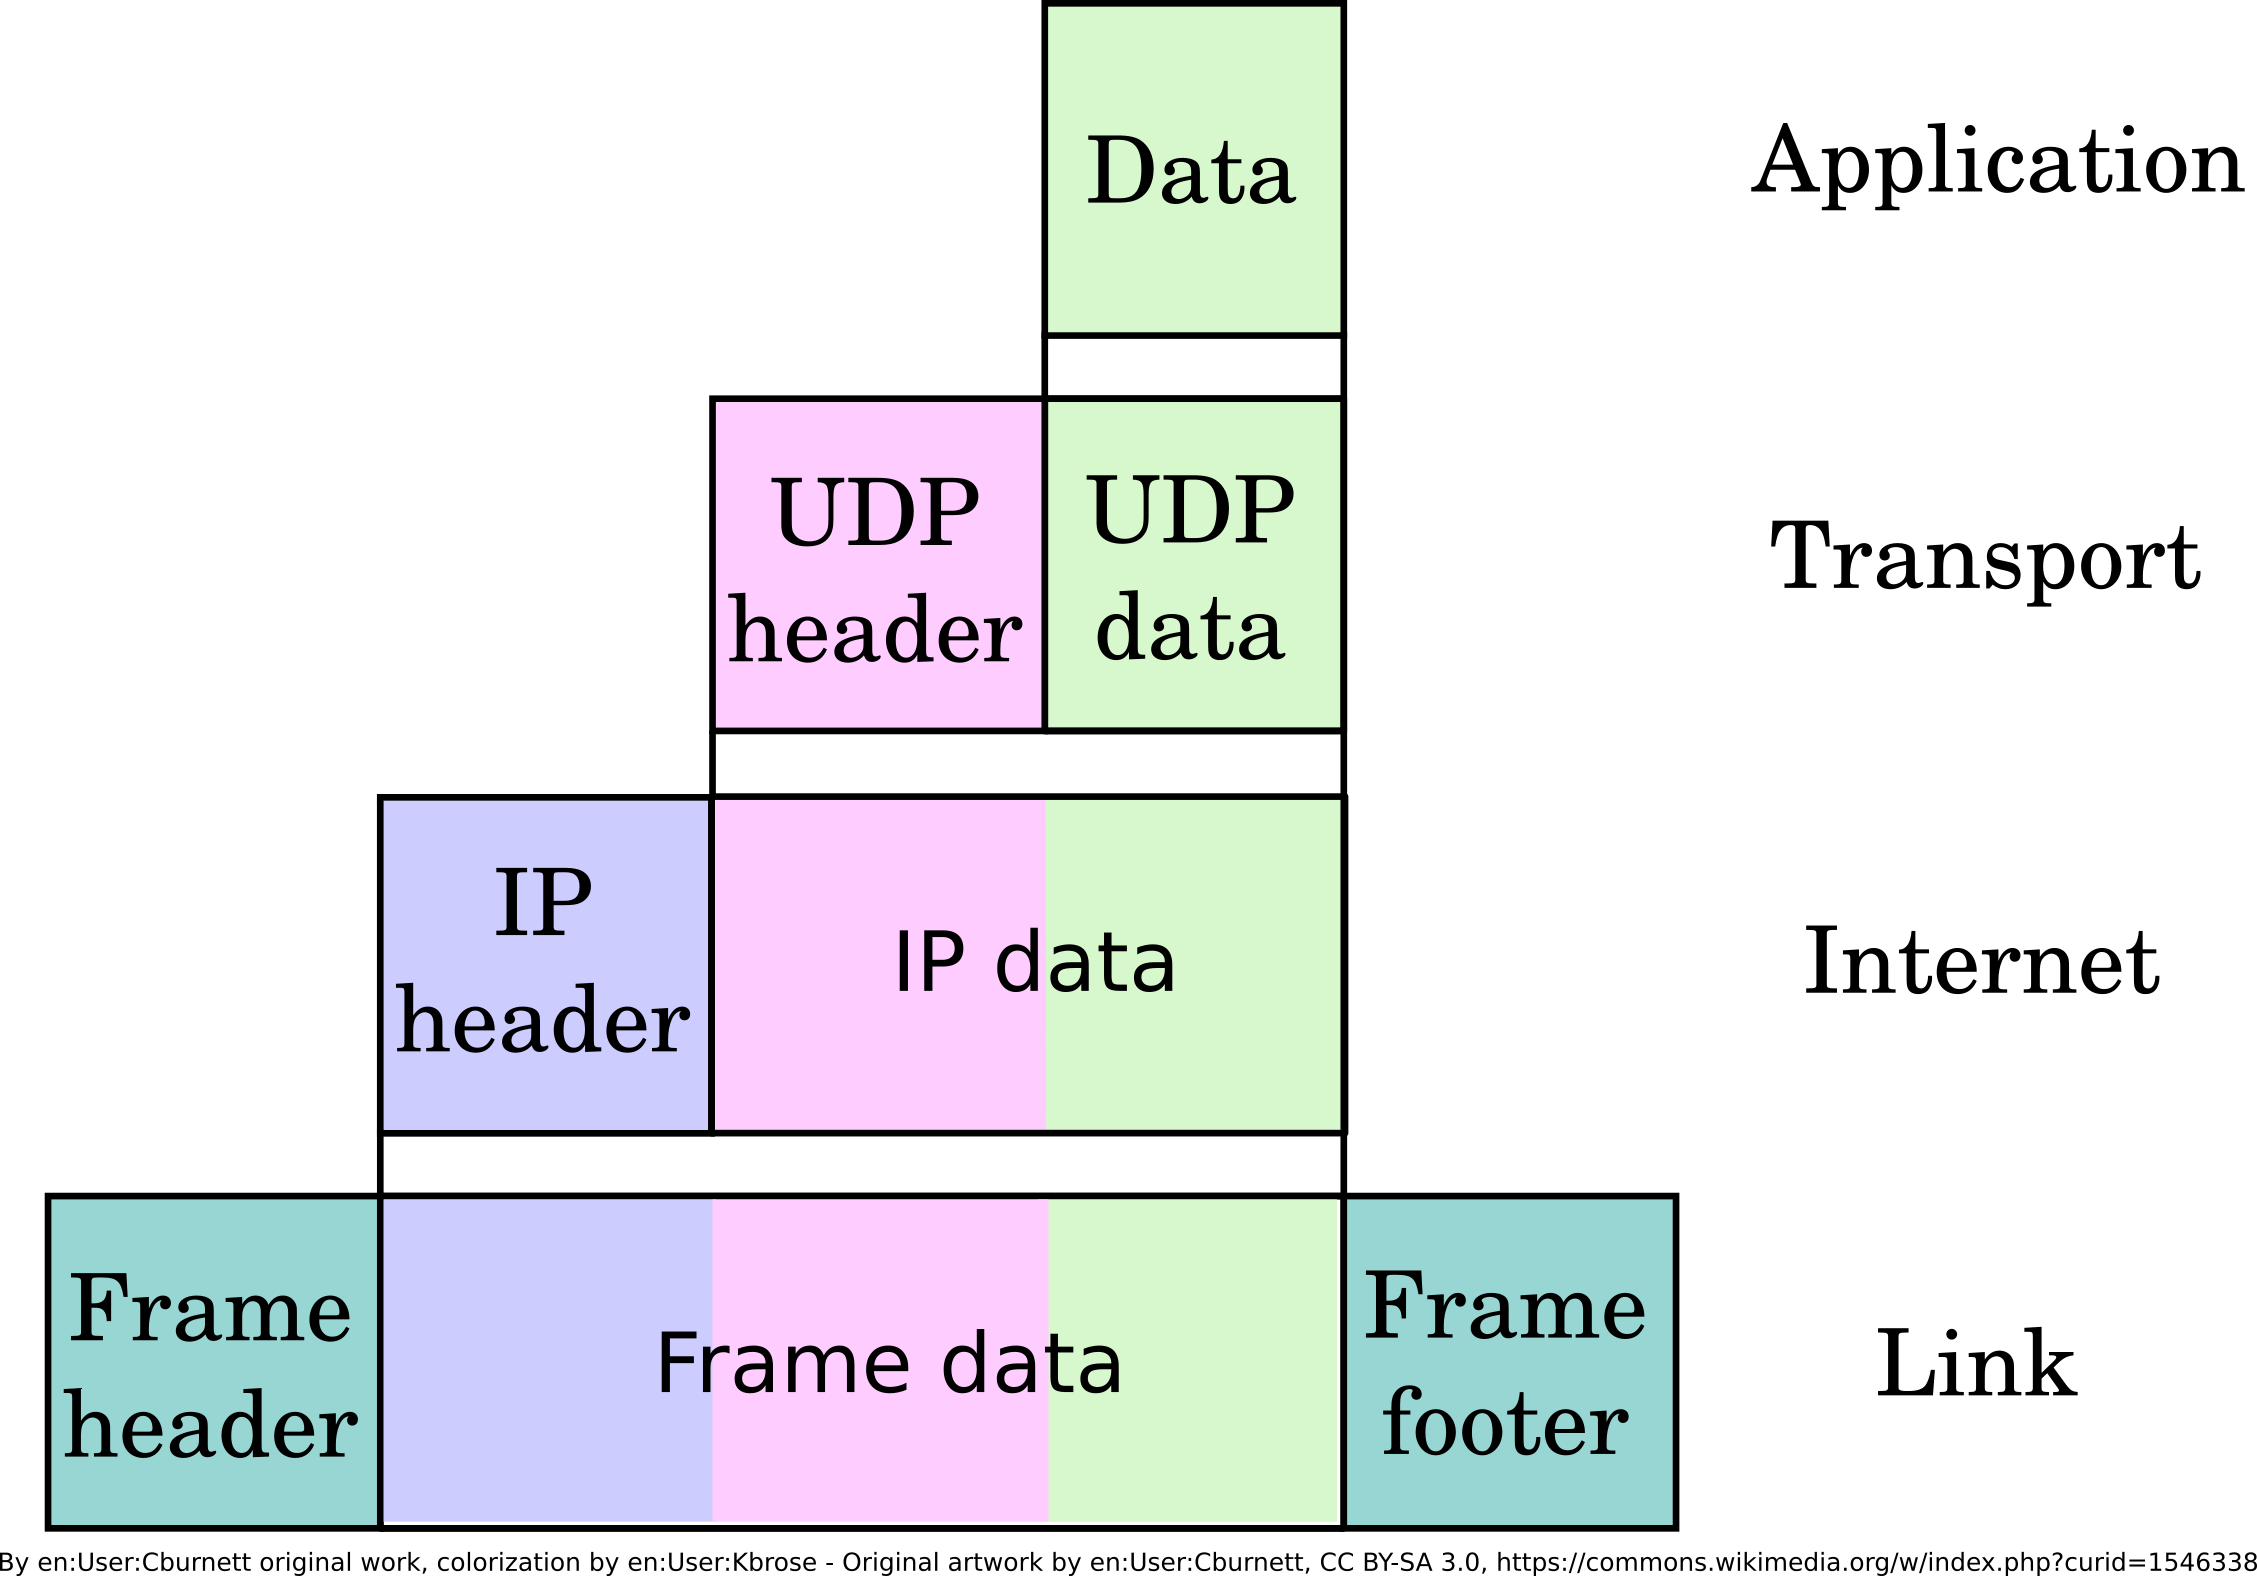
\includegraphics[width=0.9\linewidth]{UDP_encapsulation.png}
  \end{figure}
\end{frame}

\begin{frame}
  \frametitle{TCP 3}
  Zur Fehlerkorrektur werden Pakete durchnummeriert.
  \pause \vfill
  Dazu gibt es SYN und ACK Einträge im TCP-Header:\pause Das sind jeweils Zahlen von XXX bis XXX.
  \pause \vfill
  Außerdem gibt es SYN- und ACK-Pakete:

  Diese haben keine Payload, aber übermitteln im Header die SYN\# und ACK\#. % Korrekt?
  \pause \vfill
  Antwortpaket hat als ACK\# die SYN\# des vorigen Anfragepakets $\Rightarrow$ Reihenfolge der Pakete rekapitulierbar.
  \pause \vfill
  Beim Verbindungsaufbau wird mittels ACK- und SYN-Paketen ``synchronisiert'' und der Aufbau bestätigt.
\end{frame}

\begin{frame}
  \frametitle{TCP 4}
  Nummerierung der Pakete erfolgt fortlaufend. \pause Es werden SYN\# und ACK\# als Nummerierung und Bestätigung/Vorgänger geschickt.
  \vfill \pause
  ``Handshake'':
  \begin{figure}[H]
  \centering
  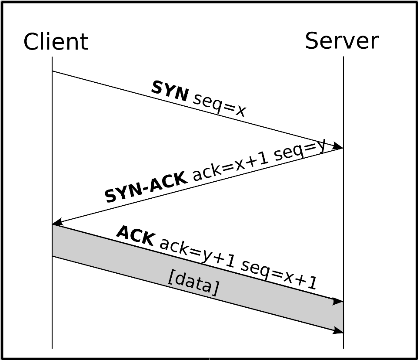
\includegraphics[width=0.6\linewidth]{tcp.png}
  \end{figure}
\end{frame}

\begin{frame}
  \frametitle{UDP}
  UDP = ``User Datagram Protocoll''
  \pause \vfill
  Benutzt auch Ports aber hat keine Fehlerkorrektur.
  \pause \vfill
  UDP hat keine Verbingung im engeren Sinne.
  \pause \vfill
  UDP ist dadurch viel schneller.
  \pause \vfill
  Wird dort benutzt, wo der Verlust von einzelnen Paketen kein Problem ist, aber Geschwindigkeit zählt.
  \pause \vfill
  Spiele, Streaming, etc.
\end{frame}

\begin{frame}
  \frametitle{Ports}
  Jeder Rechner (adressiert durch seine IP) hat sogenannte Ports, die von Anwendungen reserviert werden.
  \pause \vfill
  Beide Hosts benutzen ggf. verschiedene Ports.
  \pause \vfill
  Dadurch kann ein Rechner gleihzeitig mit mehreren Anwendungen/Servern kommunizieren.
  \pause \vfill
  Es gibt 65532 Ports, typischerweise mit 192.168.1.1:\textbf{80} bezeichnet.
  \pause \vfill
  Typische Ports: 80 -- http, \pause 22 -- ssh, \pause 443 -- https, \pause 23 -- telnet, \pause 993 -- smtp, etc.
\end{frame}

\begin{frame}
  \frametitle{ICMP}
  ICMP = ``Internet Control Message Protocol''
  \pause \vfill
  Metaprotokoll, um Informationen über Server und Verbindungen auszutauschen, insbesondere IP,TCP und UDP.
  \pause \vfill
  Beispiele für Pakete:
  \begin{itemize}
    \item Echo Request/Reply \pause
    \item Destination Network/Host/Port Unreachable \pause
    \item Time Exceeded
  \end{itemize}
  \pause \vfill
  Fehler bei ICMP Paketen werden nicht nochmal gemeldet. :-)
\end{frame}

\begin{frame}
  \frametitle{Pings}
  Ping = ``ICMP-Echo-Request/Reply''.
  \pause \vfill
  Anfrage an Server, ob dieser online ist. \pause Falls ja, sendet dieser eine Antwort.
  \pause \vfill
  Blockieren von pings ist kein Sicherheitsgewinn: Man kann auch anders herausfinden, ob ein Server online ist.
  \pause \vfill
  Typisches Beispiel:

  ``ping 8.8.8.8'' um zu schauen, ob Google erreichbar ist und damit das Internet funktioniert :-)
\end{frame}

\begin{frame}
  \frametitle{Time to live}
  Jedes IP-Paket hat eine ``Time-to-live'', eine Zahl von 0 bis 255.
  \pause \vfill
  Bei jeder Weiterleitung beim Routing (``Hop'') wird die Zahl um eins vermindert.
  \pause \vfill
  Sobald $\operatorname{TTL}=0$ ist, wird Paket ``dropped'', also gelöscht.
  \pause \vfill
  Dadurch kann ein Paket nicht in einer Endlosschleife im Routing hin- und hergeschickt werden.
  \pause \vfill
  Anwendungen: Finden von Servern des Ziels mittels \emph{traceroute}, OS-Erkennung anhand von typischen Standardwerten für TTL.
\end{frame}


\begin{frame}
  \frametitle{URLs}
  IPs kompliziert zu merken $\Rightarrow$ Nutze URLs als Adressen für Menschen.
  \pause \vfill
  Beispiel: \pause
  http://sven.musmehl.de/hacking/index.html
  \pause \vfill
  http -- Protokoll
  \pause \vfill
  de -- Topleveldomain
  \pause \vfill
  sven.musmehl.de -- Hostname
  \pause \vfill
  /hacking/ -- Unterverzeichnis/Pfad
  \pause \vfill
  index.html -- Zieldatei
  \pause \vfill
  Dahinter können noch Parameter mittels URL-Encoding übergeben werden $\Rightarrow$ Nachdem wir das http Protokoll verstanden haben.
\end{frame}

\begin{frame}
  \frametitle{URIs}
  Ganz allgemeine ``Uniform Resource Identifiers'':
  \pause \vfill
  scheme:[//[user:password@]host[:port]][/]path[?query][\#fragment]
\end{frame}

\begin{frame}
  \frametitle{DNS 1}
  Protokoll um Hostnamen und URLs in IPs aufzulösen.
  \pause \vfill
  Anstatt eine Datei (``hostfile'') mit allen IPs an alle Rechner zu schicken, werden diese Auflösungen hierarchisch verwaltet (``DNS-Einträge'') und abgefragt.
  \pause \vfill
  Beispiel: linide.sf.net. (Punkt am Ende!)
  \pause \vfill
  Anfrage an . : Was ist IP von net.?
  \pause \vfill
  Anfrage an Nameserver von net. : Was ist IP vom Nameserver von sf.net.?
  \pause \vfill
  Anfrage an Nameserver von sf.net. : Was ist IP von linide.sf.net.?
  \pause \vfill
  Danach werden ``normale'' http Anfragen und ähnliches an IP von linide.sf.net gesendet.
  \pause \vfill
  Caching-Nameserver speichern Anfragen zwischen um diese schneller zu beantworten.
\end{frame}

\begin{frame}
  \frametitle{DNS 2}
  Beispiele für DNS-Einträge:
  \pause \vfill
  A -- Symbolischer Name $\rightarrow$ IP
  \pause \vfill
  PTR -- IP $\rightarrow$ symbolischer Name (z.B.\ zur Verifikation mittels ``Reverse-Lookup'')
  \pause \vfill
  NS -- IP des Nameservers für das Subnetz der Domain
  \pause \vfill
  CNAME -- Symbolischer Name $\rightarrow$ symbolischer Name (z.B.\ für Domains bei Hostinganbietern, die keinen eigenen Server haben)
  \pause \vfill
  MX -- Symbolischer Name des Mailservers für die Domain
\end{frame}

\subsection{Internetprotokolle}

\begin{frame}
  \frametitle{HTTP 1}
  http = ``Hypertext Transfer Protocol''
  \pause \vfill
  Es gibt zwei Versionen: HTTP/1.1 und HTTP/2.
  \pause \vfill
  http ist auf Anwendungsebene und nutzt TCP auf Transportebene.
  \pause \vfill
  http ist ein Anfrage--Antwort-Protokoll für den Datenaustausch zwischen Server und Client.
  \pause \vfill
  Wichtigste http Methoden: \pause
  \begin{itemize}
    \item GET -- Anfrage zum Download von Daten \pause
    \item POST -- Anfrage zum Upload von Daten (z.B. für Skripte) \pause
    \item PUT -- Speichere Daten unter der Adresse \pause
    \item TRACE -- Gib Befehl wieder zurück (um zu vergleichen)
  \end{itemize}
\end{frame}

\begin{frame}
  \frametitle{HTTP 2}
  Beispiel:

  ``GET /index.html HTTP/1.1'' -- \pause Schicke mir die Datei ``index.html'' mittels HTTP/1.1 Standard
  \pause \vfill
  Serverantwort: \pause

{\tiny  
HTTP/1.1 200 OK \\
Date: Mon, 23 May 2005 22:38:34 GMT \\
Content-Type: text/html; charset=UTF-8 \\
Content-Encoding: UTF-8 \\
Content-Length: 138 \\
Last-Modified: Wed, 08 Jan 2003 23:11:55 GMT \\
Server: Apache/1.3.3.7 (Unix) (Red-Hat/Linux) \\
ETag: "3f80f-1b6-3e1cb03b" \\
Accept-Ranges: bytes  \\
Connection: close \\[1em]

<html> \\
<head> \\
  <title>An Example Page</title> \\
</head> \\
<body> \\
  Hello World, this is a very simple HTML document. \\
</body> \\
</html> \\
}
\end{frame}

\begin{frame}
  \frametitle{HTTP 3}
   Statuscodes (dreistellige Zahlen):
  \begin{itemize}
    \item 200 -- ``OK'' \pause
    \item 404 -- ``Not Found'' \pause
    \item 400 -- ``Bad Request'' \pause
    \item 418 -- ``I'm a teapot'' \pause
    \item 500 -- ``Internal Server Error'' \pause
    \item 502 -- ``Bad Gateway'' bei Proxys u.ä.\ 
  \end{itemize}
\end{frame}

\begin{frame}
  \frametitle{URL Encoding}
  Für viele Webanwendungen müssen Informationen in URI eingebaut werden, z.B. wie in \pause ``http://www.w3.com/form\_submit.asp?text=Das+ist+so+\%2Fmega\%3A*''
  \pause \vfill
  Reservierte Zeichen haben Bedeutung für URI, z.B. /, !, +
  \pause \vfill
  Unreservierte Zeichen können beliebig verwendet werden. $\Rightarrow$ Zusammen mit dem \% Zeichen werden ``alle'' Zeichen kodiert.
  \pause \vfill
  Beispiele:
  \begin{itemize}
    \item / -- \%2F \pause
    \item + -- \%2A \pause
    \item ü -- \%C3\%BC
  \end{itemize}
  \pause \vfill
  $\Rightarrow$ Man kann oft den Input für Webseiten manuell in der URL manipulieren!
\end{frame}

\begin{frame}
  \frametitle{HTTPS}
  
\end{frame}

\begin{frame}
  \frametitle{SMTP, POP3, IMAP4}

\end{frame}

\begin{frame}
  \frametitle{FTP und SFTP}
  
\end{frame}

\begin{frame}
  \frametitle{SSH und SCP}
  
\end{frame}

\begin{frame}
  \frametitle{Whois}
  
\end{frame}

\section{Wichtigste Systeme im Internet}

\begin{frame}
  \frametitle{Apache und Nginx}
  
\end{frame}

\begin{frame}
  \frametitle{PHP und Javascript}
    
\end{frame}

\begin{frame}
  \frametitle{SQL}
  
\end{frame}

\section{Wichtige Kommandozeilenwerkzeuge}

\subsection{Kommunikation über Netzwerke}

\begin{frame}
  \frametitle{Curl und wget}
  
\end{frame}

\begin{frame}
  \frametitle{Netcat}
  
\end{frame}

\begin{frame}
  \frametitle{Telnet}
  
\end{frame}

\begin{frame}
  \frametitle{SSH und SCP}
  
\end{frame}

\begin{frame}
  \frametitle{tcpdump}
  
\end{frame}

\begin{frame}
  \frametitle{Wireshark}
  
\end{frame}

\subsection{Reconnaissance}

\begin{frame}
  \frametitle{Host}
  
\end{frame}

\begin{frame}
  \frametitle{Whois}
  
\end{frame}

\begin{frame}
  \frametitle{Ping}
  
\end{frame}

\begin{frame}
  \frametitle{Nmap}
  
\end{frame}

\begin{frame}
  \frametitle{Nmap Resultate}
  
\end{frame}

\begin{frame}
  \frametitle{Nmap OS Erkennung}
  
\end{frame}

\begin{frame}
  \frametitle{Traceroute}
  
\end{frame}

\section{Verschiedene Attacken}

\subsection{Allgemeines Vorgehen}

\begin{frame}
  \frametitle{Vorgehen}
  
\end{frame}

\begin{frame}
  \frametitle{Ziele}
  
\end{frame}

\subsection{ARP Spoofing}

\begin{frame}
  \frametitle{ARP}
  
\end{frame}

\begin{frame}
  \frametitle{Wireshark mit ARP Spoofing}
  
\end{frame}

\subsection{WEP Verschlüsselung}

\begin{frame}
  \frametitle{WEP-RC4}
  
\end{frame}

\begin{frame}
  \frametitle{Aircrack}
  
\end{frame}

\subsection{Websites}

\begin{frame}
  \frametitle{Session IDs}
  
\end{frame}

\begin{frame}
  \frametitle{Cookies}
  
\end{frame}

\begin{frame}
  \frametitle{Beispiel: PhPBB}
  
\end{frame}

\begin{frame}
  \frametitle{SQL Injection}
  
\end{frame}

\subsection{DNS Tunneling}

\begin{frame}
  \frametitle{Iodine}
  
\end{frame}

\begin{frame}
  \frametitle{DNS Tunneling}
  
\end{frame}


\end{document}
